\documentclass{beamer}

\usetheme{Antibes}
\useoutertheme[subsection=false]{miniframes}

%\usetheme{split}
%\usetheme{Madrid}
%\usetheme{Berkeley}

\usecolortheme[RGB={120,0,0}]{structure}
\setbeamertemplate{blocks}[rounded][shadow=true]
\setbeamertemplate{footline}[frame number]
\setbeamersize{text margin left=.5cm,text margin right=.5cm} 
\usepackage[utf8]{inputenc}   % pacote para acentuao
\usepackage{graphicx}
\usepackage{subcaption}

%\usepackage[latin1]{inputenc}

\beamertemplateballitem
\beamertemplatenavigationsymbolsempty

\begin{document}

\title{Assessing the Computation and Communication Overhead of Linux Containers for HPC Applications}
\author{
\large 
\underline{Guilherme R. Alles}, Lucas M. Schnorr, Alexandre Carissimi\\
\small
\vspace*{0.5cm}
Instituto de Informática\\ Universidade Federal do Rio Grande do Sul \\\medskip

\includegraphics[width=.15\textwidth]{cnpq.png}%
\hspace{.5 cm}%
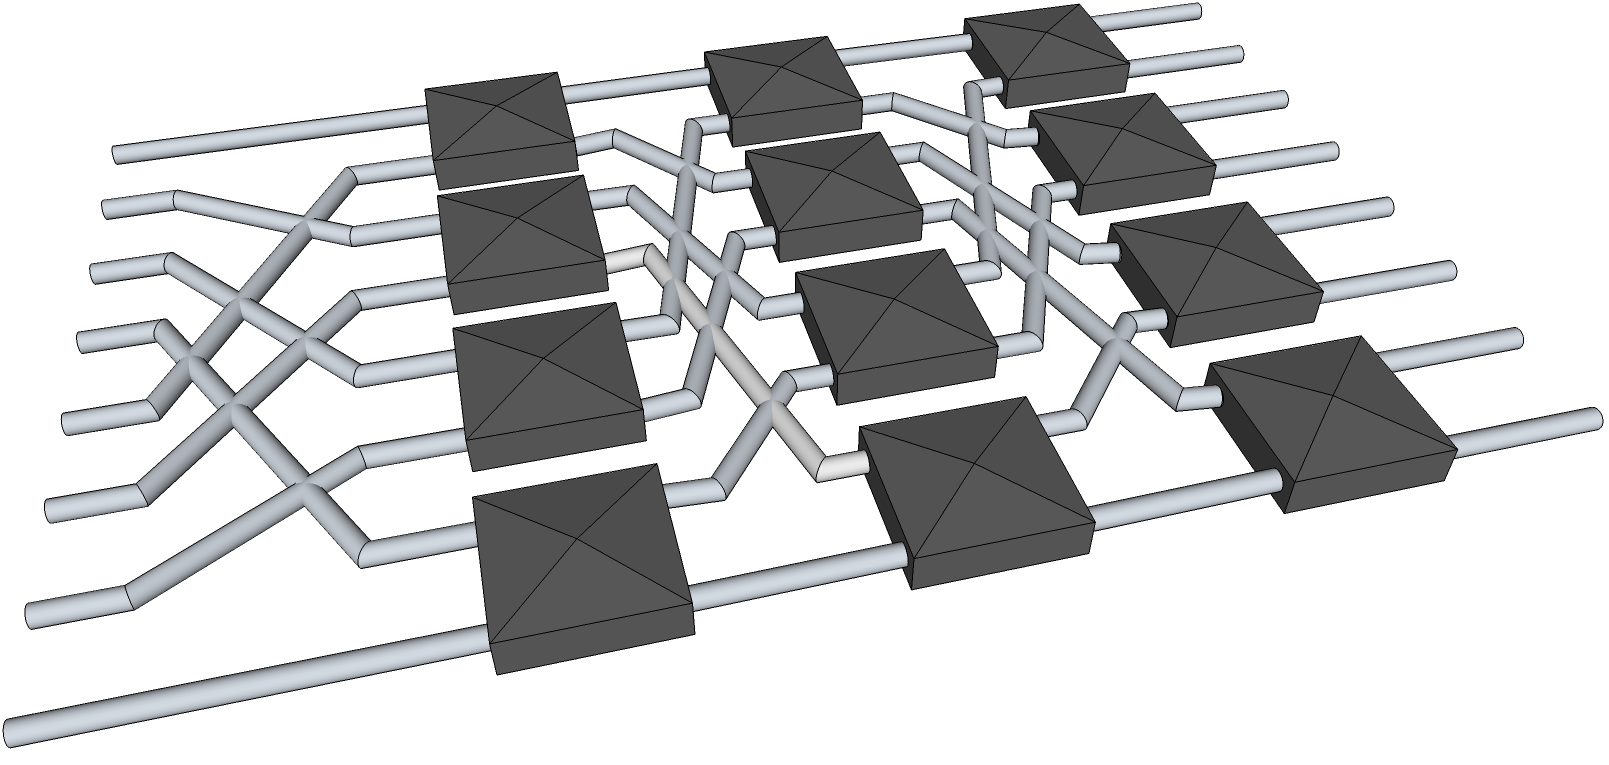
\includegraphics[width=.15\textwidth]{gppd-logo.png} \\\vspace{-.5cm}
}
\date{Simpósio de Sistemas Computacionais de Alto Desempenho\\
  2 de outubro de 2018}

\frame{\titlepage}

\section*{Introduction and Objectives}
\frame{\frametitle{Introduction}
    \begin{itemize}
        \item HPC clusters are \textbf{highly heterogeneous}
        \begin{itemize}
            \item Hardware configurations, software stacks, usage policies...
        \end{itemize}
        \pause
        \vspace*{0.3cm}
        \item Designing experiments for portability requires investing time
        \begin{itemize}
            \item Operating system specifics
            \item Dependency management
        \end{itemize}
        \pause
        \vspace*{0.3cm}
        \item What if someone wants to reproduce your experiments?
    \end{itemize}
}

\frame{\frametitle{Introduction}
    Possible solution: virtual machines! \pause But...
    \begin{itemize}
        \item Requires a \textbf{hypervisor}. Which one?
        \begin{itemize}
            \item Type 1, Type 2, paravirtualization
            \item What if different clusters support different hypervisors?
        \end{itemize}
        \item Multi-gigabyte system images
        \item \textbf{Overhead}
    \end{itemize}
}

\frame{\frametitle{Introduction}
    Why can't we use Linux Containers?
    \begin{itemize}
        \pause
        \vspace*{0.2cm}
        \item No hypervisor overhead
        \pause
        \vspace*{0.2cm}
        \item Images take much less space
        \pause
        \vspace*{0.2cm}
        \item APIs integrated in the Linux Kernel
        \pause
        \vspace*{0.2cm}
        \item Flexibility yield performance gains at a small development cost
    \end{itemize}
}

\frame{\frametitle{Objectives}
        Measure \textbf{viability} of applying container technology to HPC
        \pause
        \begin{itemize}
            \item Computation overhead (application makespan)
            \item Communication overhead (latency/bandwidth)
        \end{itemize}
        \pause
        \vfill
        Contrast two popular container environments and their \textbf{workflows}
        \begin{itemize}
            \item Docker
            \item Singularity
        \end{itemize}
    \vfill
    {\hspace{2cm}
\includegraphics[width=.35\textwidth]{docker-logo.png}\hfill%

\includegraphics[width=.1\textwidth]{singularity-logo.png}\hspace{2cm}}
}

\frame{\frametitle{Outline}\tableofcontents[hideallsubsections]}

\section{Linux Containers}
\frame{\frametitle{Linux Containers}
  \vspace*{0.2cm}
  \centering
  \begin{columns}
    \begin{column}{0.5\textwidth}
      OS level virtualization

      \bigskip
      
      Build into the Linux Kernel
      \begin{itemize}
      \item \textbf{Resource control} (cgroups)
      \item \textbf{Isolation} (namespaces)
      \end{itemize}
    \end{column}
    \begin{column}{0.5\textwidth}
      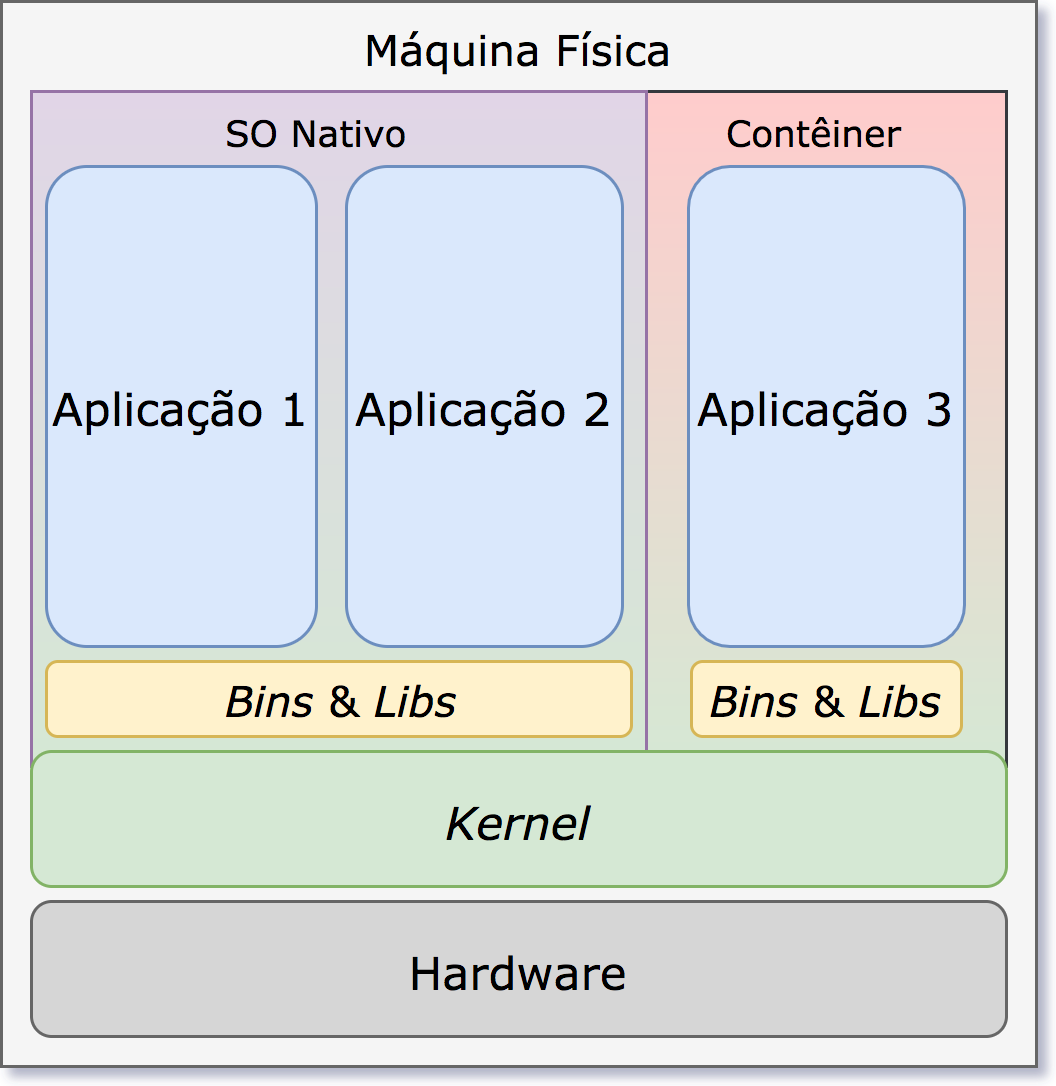
\includegraphics[width=\linewidth]{conteineres.png}
    \end{column}
  \end{columns}
}

\frame{\frametitle{Docker}
    \vspace*{-0.7cm}
    \begin{figure}
        \centering
        
\includegraphics[width=.5\textwidth]{docker-logo.png}
    \end{figure}
    \vspace*{-0.2cm}
    \begin{itemize}
    \item Widely used in the industry (for microservices virtualization)
    \item Standard in cloud IaaS providers such as AWS, GCP and Azure
      \pause\vfill
    \item Enforces virtualization for all six Linux Kernel namespace
      \begin{itemize}
      \item \emph{mount} (filesystem tree and mounts)
      \item \emph{PID} (process IDs)
      \item \emph{UTS} (host name and domain name)
      \item \emph{\bf network} (devices, ports, routing tables, firewall)
      \item \emph{IPC} (inter-process communication resources)
      \item \emph{\bf user} (unpriviliged, added in Linux 3.8)
      \end{itemize}
      \pause
    \item Implications on the use case (elaborate on that)
    \end{itemize}
}

\frame{\frametitle{Singularity}
    \vspace*{-0.5cm}
    \begin{figure}
        \centering
        
\includegraphics[width=.1\textwidth]{singularity-logo.png}
    \end{figure}
    \vspace*{-0.2cm}
    \begin{itemize}
        \item Linux Containers for HPC
        \vspace*{0.2cm}
        \item Alternative to Docker drawbacks for shared environments
        \pause
        \vspace*{0.2cm}
        \item Objective: \textbf{secure} container environment for HPC clusters
        \pause
        \vspace*{0.2cm}
        \item Virtualizes \textbf{only the necessary namespaces}. Everything else is kept optional.
        \begin{itemize}
            \item \textbf{file system}
        \end{itemize}
    \end{itemize}
}

\section{Experimental Design}
\frame{\tableofcontents[currentsection,hideothersubsections]}

\frame{\frametitle{Testbed}
    \begin{itemize}
        \item Grid5000's Graphene clusters
        \begin{itemize}
            \item Intel Xeon X3340, 4 cores @ 2.53GHz
            \item 16GB DDR3 RAM
            \item Gigabit Ethernet interconnect
        \end{itemize}
        \pause
        \vspace*{0.5cm}
        \item Debian 9 (\textit{stretch}) Linux
        \begin{itemize}
            \item Containers running on top of the native environment
            \item Docker containers connected through Docker Swarm \textit{overlay}
            \begin{itemize}
                \item Necessary because of \textbf{PID} and \textbf{network} virtualization
                \item Allows addressing MPI processes
            \end{itemize}
        \end{itemize}
    \end{itemize}
}

\frame{\frametitle{Workload}
    NAS Parallel Benchmarks
    \begin{itemize}
        \item Synthetic workload for baseline purposes
        \item EP (\textit{embarrassingly parallel}) Kernel
        \begin{itemize}
            \item CPU bound scenario
            \item Low communication between workers
            \item Workload size B
        \end{itemize}
    \end{itemize}
    \pause
    \vspace*{0.2cm}
    Ondes3D
    \begin{itemize}
        \item Seismic waves propagation simulation
        \item Load imbalance, frequent communication
        \begin{itemize}
            \item Workload: default test case + Ligurian
        \end{itemize}
    \end{itemize}
    \vspace*{0.2cm}
    \pause
    Ping-Pong benchmark
    \begin{itemize}
        \item Network latency
    \end{itemize}
}

\section{Results}
\frame{\tableofcontents[currentsection,hideothersubsections]}

\frame{\frametitle{Results - NAS EP}
    \begin{figure}
        \centering
        \begin{subfigure}{.45\textwidth}
            \hspace*{-1.2cm}
            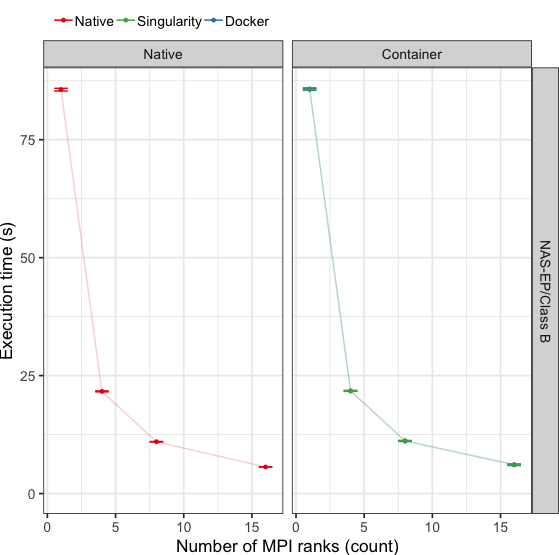
\includegraphics[width=1.2\textwidth]{nas-ep-raw.png}
        \end{subfigure}
        \pause
        \begin{subfigure}{.45\textwidth}
        \hspace*{0.2cm}
            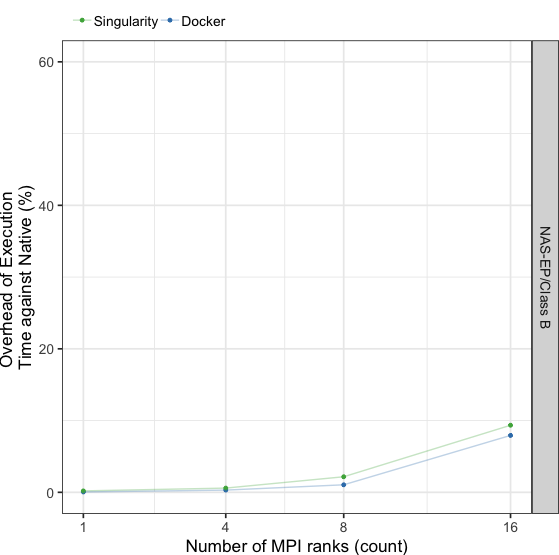
\includegraphics[width=1.2\textwidth]{nas-ep-overhead.png}
        \end{subfigure}
    \end{figure}
}

\frame{\frametitle{Results - Ondes3D Default}
    \begin{figure}
        \centering
        \begin{subfigure}{.45\textwidth}
            \hspace*{-1.2cm}
            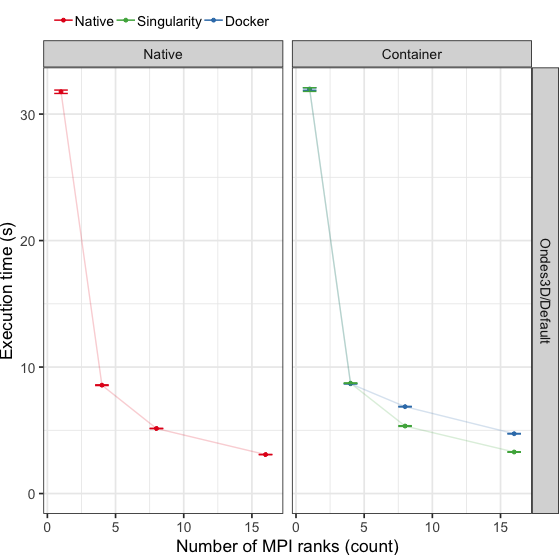
\includegraphics[width=1.2\textwidth]{ondes3d-default-raw.png}
        \end{subfigure}
        \pause
        \begin{subfigure}{.45\textwidth}
        \hspace*{0.2cm}
            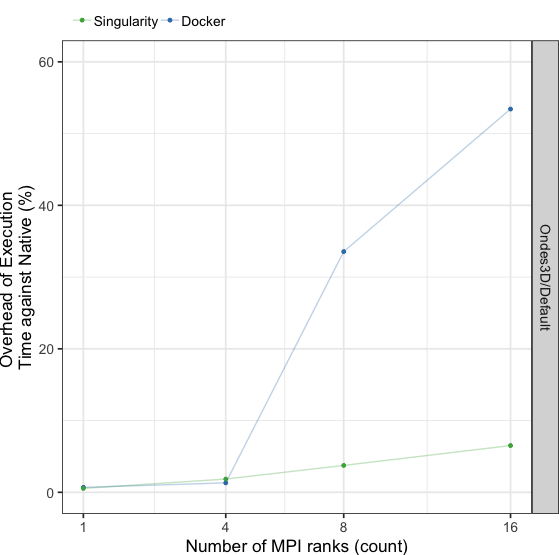
\includegraphics[width=1.2\textwidth]{ondes3d-default-overhead.png}
        \end{subfigure}
    \end{figure}
}

\frame{\frametitle{Results - Ondes3D Ligurian}
    \begin{figure}
        \centering
        \begin{subfigure}{.45\textwidth}
            \hspace*{-1.2cm}
            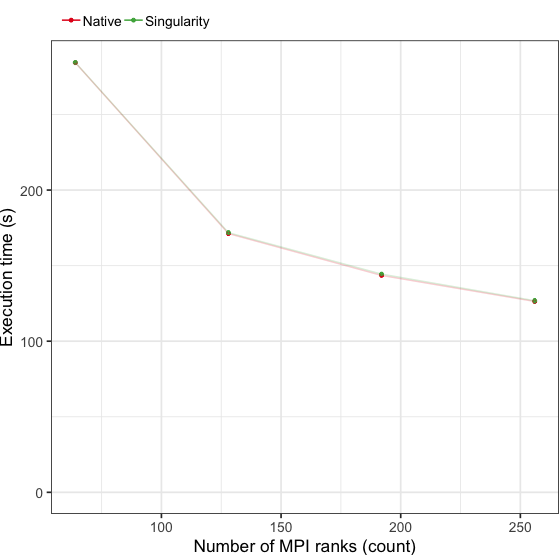
\includegraphics[width=1.2\textwidth]{ondes3d-ligurian-raw.png}
        \end{subfigure}
        \pause
        \begin{subfigure}{.45\textwidth}
        \hspace*{0.2cm}
            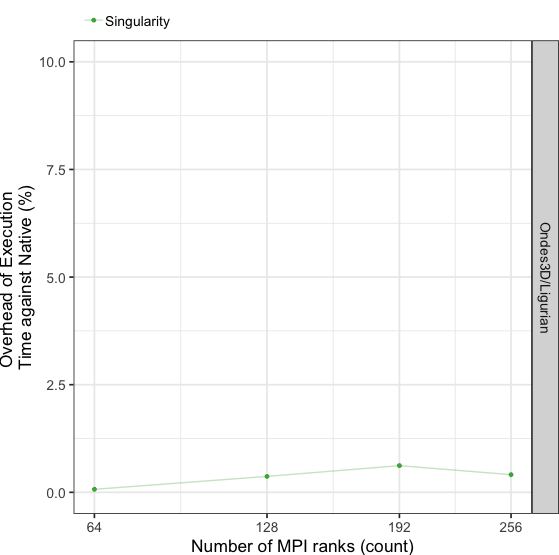
\includegraphics[width=1.2\textwidth]{ondes3d-ligurian-overhead.png}
        \end{subfigure}
    \end{figure}
}

\frame{\frametitle{Results - Ping Pong}
    \begin{figure}
        \centering
        \vspace*{-0.2cm}
        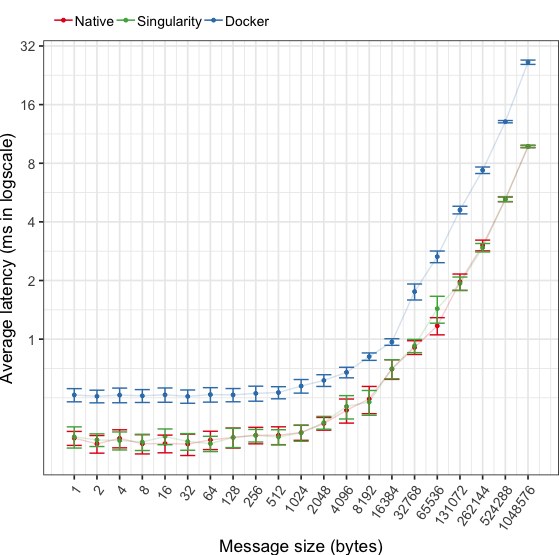
\includegraphics[width=0.65\textwidth]{network-latency-raw.png}
    \end{figure}
}

\frame{\frametitle{Results - Alpine Linux}
    \begin{figure}
        \centering
        \begin{subfigure}{.45\textwidth}
            \hspace*{-1.2cm}
            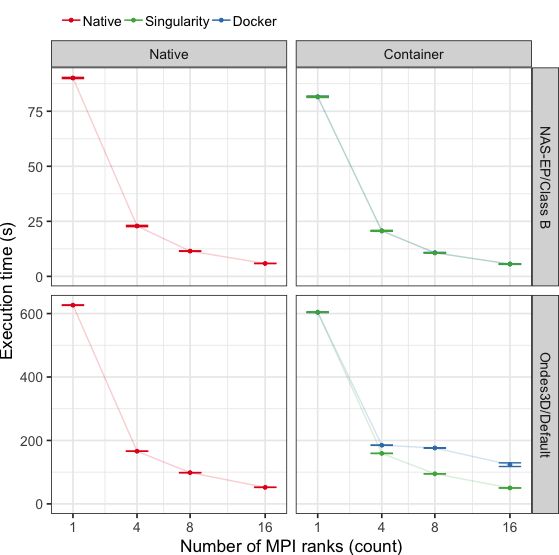
\includegraphics[width=1.2\textwidth]{alpine-nas-ondes3d-raw.png}
        \end{subfigure}
        \pause
        \begin{subfigure}{.45\textwidth}
        \hspace*{0.2cm}
            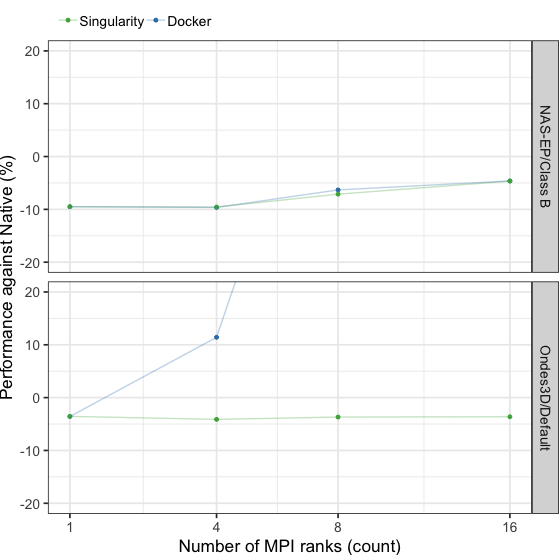
\includegraphics[width=1.2\textwidth]{alpine-nas-ondes3d-overhead.png}
        \end{subfigure}+
    \end{figure}
}

\section{Conclusions and Future Work}
\frame{\tableofcontents[currentsection,hideothersubsections]}

\frame{\frametitle{Conclusions}
    \begin{itemize}
        \item Containers are a viable way of virtualizing an HPC environment
        \pause
        \item Computational overhead is negligible in most use cases
        \pause
        \item Communication overhead is significant, especially in the Docker environment
        \begin{itemize}
            \item Virtualization of the \textbf{network} namespace impacts MPI workloads
        \end{itemize}
        \pause
        \item Performance gains are attainable by \textbf{fine tuning} the execution environment
    \end{itemize}
}

\frame{\frametitle{Future Work}
    \begin{itemize}
        \item Further investigate Docker Swarm scalability
        \begin{itemize}
            \item Increased latency
            \item Failure to spawn a larger number of containers
        \end{itemize}
        \pause
        \vspace*{0.3cm}
        \item Explore container compatibility with other devices
        \begin{itemize}
            \item GPU
            \item InfiniBand
        \end{itemize}
    \end{itemize}
}

\end{document}
